\documentclass[tikz,border=10pt]{standalone}
\begin{document}
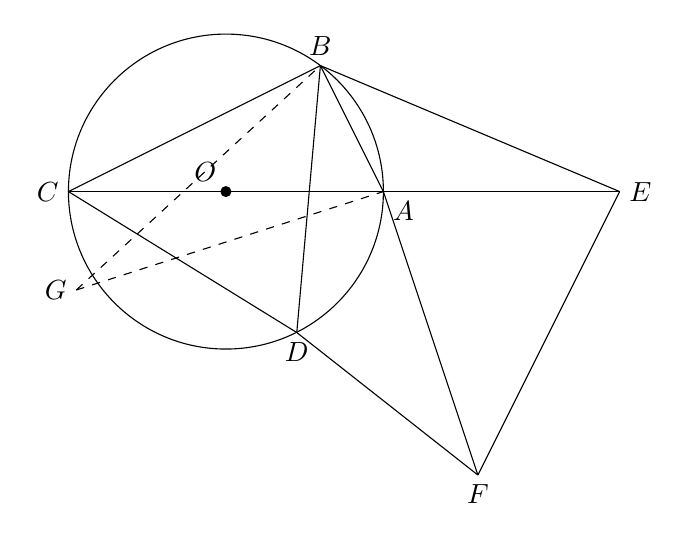
\begin{tikzpicture}[scale=1]
% circle
\draw (0,0) circle (2);

% coordinates
\coordinate (O) at (0,0);
\coordinate (C) at (-2,0);
\coordinate (A) at (2,0);
\coordinate (E) at (5,0);
\coordinate (B) at (1.2,1.6);
\coordinate (D) at (0.9,-1.79);
\coordinate (G) at (-1.9,-1.25);
\coordinate (F) at (3.2,-3.6);

% circle and dashed lines
\draw[dashed] (G) -- (B);
\draw[dashed] (G) -- (A);

% solid edges
\draw (C) -- (E);
\draw (C) -- (B);
\draw (B) -- (D);
\draw (B) -- (A);
\draw (C) -- (D);
\draw (A) -- (F);
\draw (D) -- (F);
\draw (B) -- (E);
\draw (E) -- (F);

% points and labels
\fill (O) circle (2pt);
\node[above left] at (O) {$O$};
\node[left] at (C) {$C$};
\node[below right] at (A) {$A$};
\node[right] at (E) {$E$};
\node[above] at (B) {$B$};
\node[below] at (D) {$D$};
\node[left] at (G) {$G$};
\node[below] at (F) {$F$};
\end{tikzpicture}
\end{document}
